\section{Desafios no desenvolvimento Android}

% No desenvolvimento Android, uma tela é composta basicamente por dois arquivos, uma classe Java responsável pela criação da tela e responder aos eventos do usuário e um recurso de \textit{layout}, arquivo XML responsável pela criação da interface visual (\acl{UI} - \acs{UI}).

\textit{Activity} é um dos principais componentes de aplicativos Android. Ela representa uma tela com interface do usuário (\acl{UI} - \acs{UI}) pelo qual o usuário pode interagir através de botões, listagens, caixas de entrada de textos, dentre outros. Para implementar uma \textit{Activity} é necessário criar uma classe derivada de \texttt{Activity} e sobrescrever alguns métodos herdados, chamados de métodos de retorno. O principal método de retorno é o \textit{onCreate}, entre suas responsabilidades está a criação da tela e configuração da \acs{UI}. O Código-Fonte \ref{lst:BasicActivity} apresenta o código mínimo para a criação de uma \textit{Activity}, na linha 5 temos o código responsável pela configuração da \acs{UI} que indica o recurso de \textit{layout} ``main\_activity''.

\begin{lstlisting}[
  language=Java, 
  caption={Código mínimo para a criação de uma \textit{Activity}}, 
  label={lst:BasicActivity}
]
public class MainActivity extends Activity {
  @Override
  public void onCreate(Bundle savedInstanceState) {
      super.onCreate(savedInstanceState);
      setContentView(R.layout.main_activity);
  }
}
\end{lstlisting}

A \acs{UI} de uma \textit{Activity} é construída por meio de recursos de \textit{layout}, arquivos XML cujo as \textit{tags} provém do kit de desenvolvimento Android (\acl{SDK} - \acs{SDK}) e representam \textit{Views} ou \textit{ViewGroups}. O Código-Fonte \ref{lst:SimpleLayout} apresenta um recurso de \textit{layout} com duas \textit{Views} e um \textit{ViewGroup}. As \textit{Views} são um \textit{TextView}, que representa uma caixa de entrada de texto e um \textit{Button}, que representa um botão. Essas duas \textit{Views} estão contidas dentro do \textit{ViewGroup} \textit{LinearLayout}, que as organiza verticalmente. 


\begin{lstlisting}[
  language=XML, 
  caption={Exemplo de recurso de \textit{layout} com um campo de entrada de texto e um botão organizados um abaixo do outro.}, 
  label={lst:SimpleLayout}
]
<?xml version="1.0" encoding="utf-8"?>
<LinearLayout ...
    android:layout_width="fill_parent"
    android:layout_height="fill_parent"
    android:orientation="vertical">

    <TextView android:id="@+id/text"
        android:layout_width="wrap_content"
        android:layout_height="wrap_content"
        android:text="Um TextView" />

    <Button android:id="@+id/button"
        android:layout_width="wrap_content"
        android:layout_height="wrap_content"
        android:text="Um Button" />
</LinearLayout>
\end{lstlisting}

Os códigos apresentados são bem simples, mas comumente, estas telas e \acs{UI}s tendem a ser bem mais robustas e ricas de informações e interatividade. São em contextos como esses que os desafios no desenvolvimento da camada de apresentação Android surgem. \acs{UI}s ricas e robustas podem significar muitas \textit{Views} e \textit{ViewGroups}, resultando em recursos de \textit{layout} grandes e complexos. E ainda, quanto mais ricas e robustas são as \acs{UI}s, mais provavelmente o código das \textit{Activities} correspondentes também serão grandes e complexos, pois são pelas \textit{Activities} que \textit{Views} e \textit{ViewGroups} conseguem interagir com o usuário, também são pelas \textit{Activities} que os dados chegam até a \acs{UI} e vice-versa, dentre muitas outras responsabilidades que tendem a ficar com as \textit{Activities}.

\subsection{Ciclo de Vida}

Toda \textit{Activity}, bem como outros componentes Android, possui um ciclo de vida. O ciclo de vida de um componente é composto por um conjunto de métodos de retorno, que por sua vez, são métodos invocados pelo Android em uma ordem específica \cite{AndroidActivities2016}. Os componentes da camada de apresentação Android possuem ciclos de vida mais extensos, e portanto, mais complexos. 

Como exemplo, na Figura \ref{fig:android-lifecycles} apresentamos o ciclo de vida de três componentes Android: \textit{Activities} e \textit{Fragments}, ambos relacionados à camada de apresentação, e \textit{Services}, componente usado para longos processamento em segundo plano. Os métodos de retorno são representados pelos retângulos em cinza. É possível observar que \textit{Activities} e \textit{Fragments} possuem respectivamente sete e onze métodos de retorno enquanto que \textit{Services} possuem apenas quatro.

\begin{figure*}[!htb]
\centering
  \begin{subfigure}[b]{.33\textwidth}
    \centering
    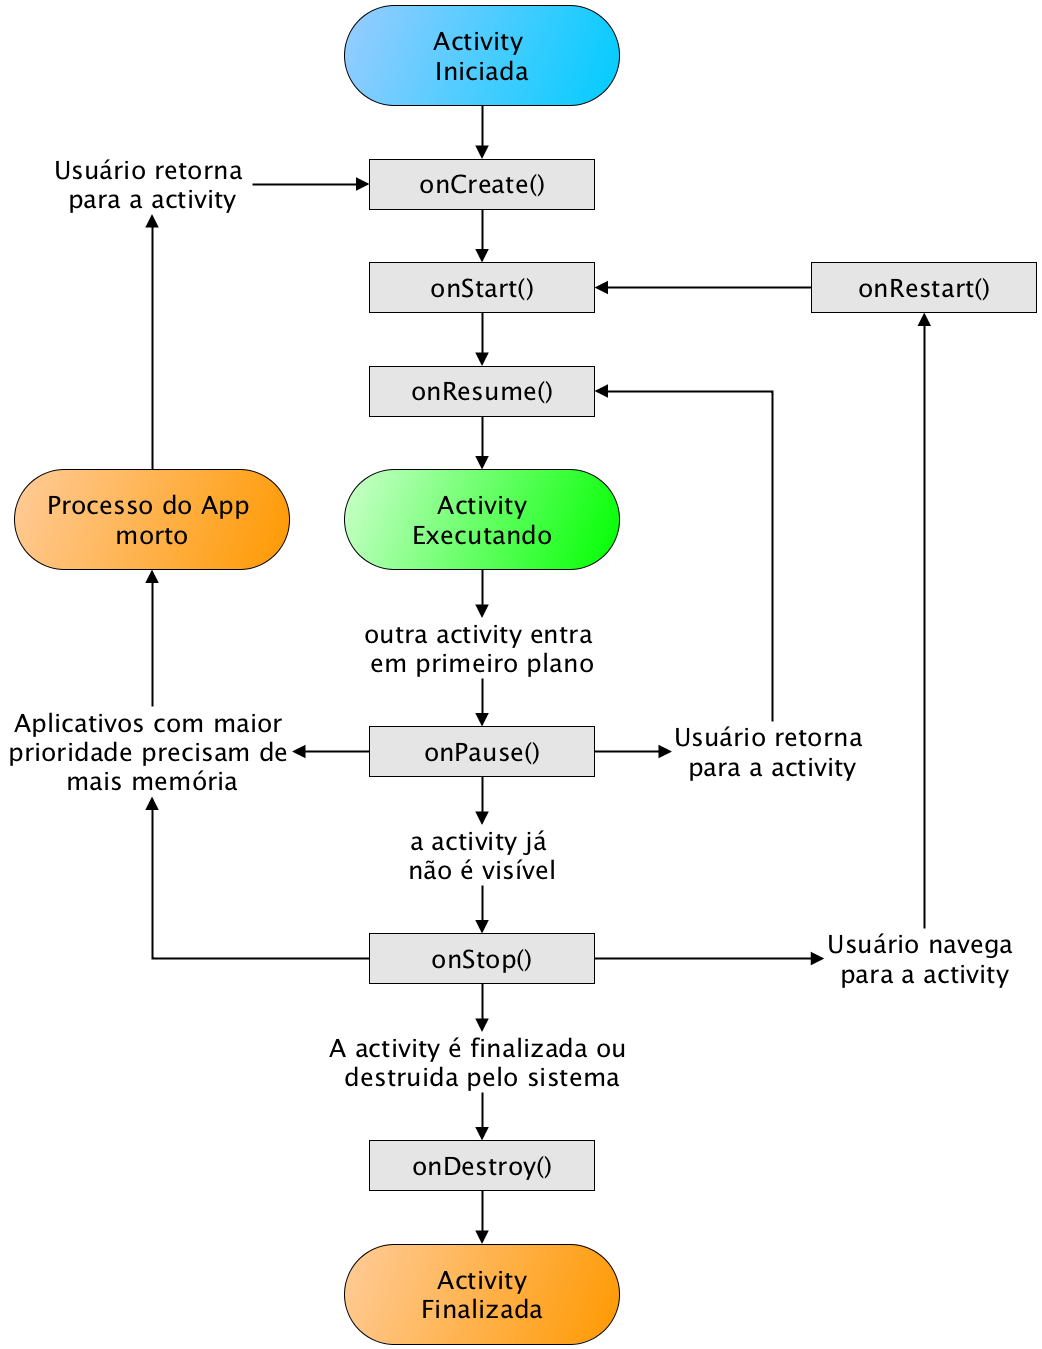
\includegraphics[width=1\textwidth]{activity-ciclodevida.png}
    \caption{\textit{Activity} (camada de apresentação).}
    \label{fig:activity-lifecycle}
  \end{subfigure}
  \begin{subfigure}[b]{.33\textwidth}
    \centering
    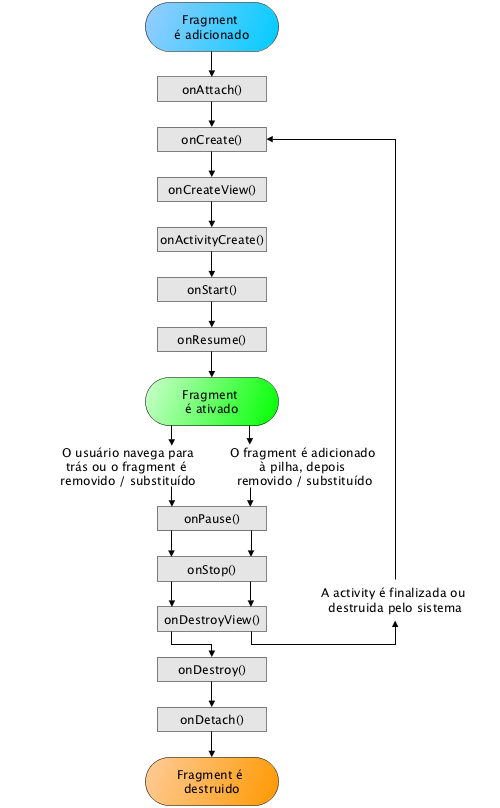
\includegraphics[width=1\textwidth]{fragment-ciclodevida.png}
    \caption{\textit{Fragment} (camada de apresentação).}
    \label{fig:activity-lifecycle}
  \end{subfigure}
  \begin{subfigure}[b]{.33\textwidth}
    \centering
    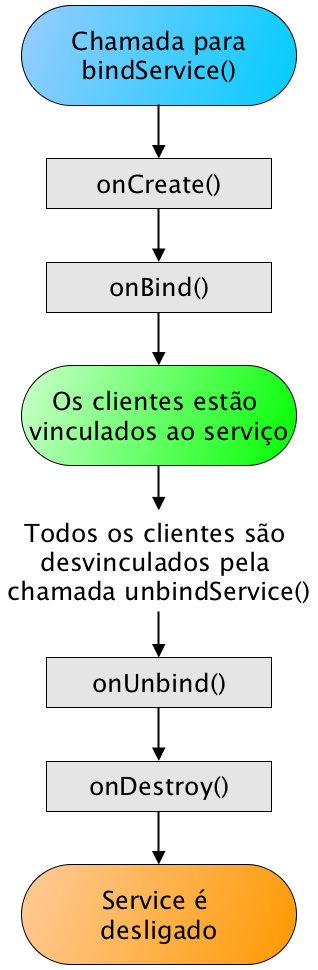
\includegraphics[width=1\textwidth]{service-ciclodevida.png}
    \caption{\textit{Services} (processamento).}
    \label{fig:service-lifecycle}
  \end{subfigure}% 
\caption{Comparativo do ciclo de vida de componentes Android que pertencem e não pertencem à camada de apresentação.}
\label{fig:android-lifecycles}
\vspace{-.5cm} 
\end{figure*}

% \begin{lstlisting}[
%   language=Java, 
%   caption={Exemplo de código para a criação de uma \textit{Activity}}, 
%   label={lst:Activity}
% ]
% public class MainActivity extends Activity {
%   @Override
%   public void onCreate(Bundle savedInstanceState) {
%       super.onCreate(savedInstanceState);
%       setContentView(R.layout.main_activity);
%       // ...
%   }
%   @Override
%   protected void onStart() {
%       super.onStart();
%       // ...
%   }
%   @Override
%   protected void onResume() {
%       super.onResume();
%       // ...
%   }
%   @Override
%   protected void onPause() {
%       super.onPause();
%       // ...
%   }
%   @Override
%   protected void onStop() {
%       super.onStop();
%       // ...
%   }
%   @Override
%   protected void onDestroy() {
%       super.onDestroy();
%       // ...
%   }
% }
% \end{lstlisting}
